
\chapter{Implementing custom analysis pipelines}
\label{custom}

All offered analysis tools provided by the MGX platform are implemented as workflows
for the Conveyor\cite{CONVEYOR} workflow engine developed by B. Linke. Within Conveyor,
tools are provided as so-called ''nodes'', which resemble individual processing steps
and which are used to implement novel analysis methods by simply arranging and connecting
them into a larger workflow. Conveyor currently includes plugins providing typical
bioinformatics tools like BLAST or HMMer, but has recently been extended with dedicated
plugins aimed at metagenome analysis, like MetaCV, MetaPhyler or MetaPhlAn, which all
perform taxonomic analysis.
A dedicated Conveyor plugin provides access to MGX data structures, thereby enabling the
analysis of metagenomes stored in the MGX system with processing tools provided by Conveyor
itself.
While workflow definitions are stored in a XML-based format, a graphical user interface,
the Conveyor Designer (\ref{designer}), enables users to implement new analysis by simply
placing and connecting nodes.

\begin{figure}[H]
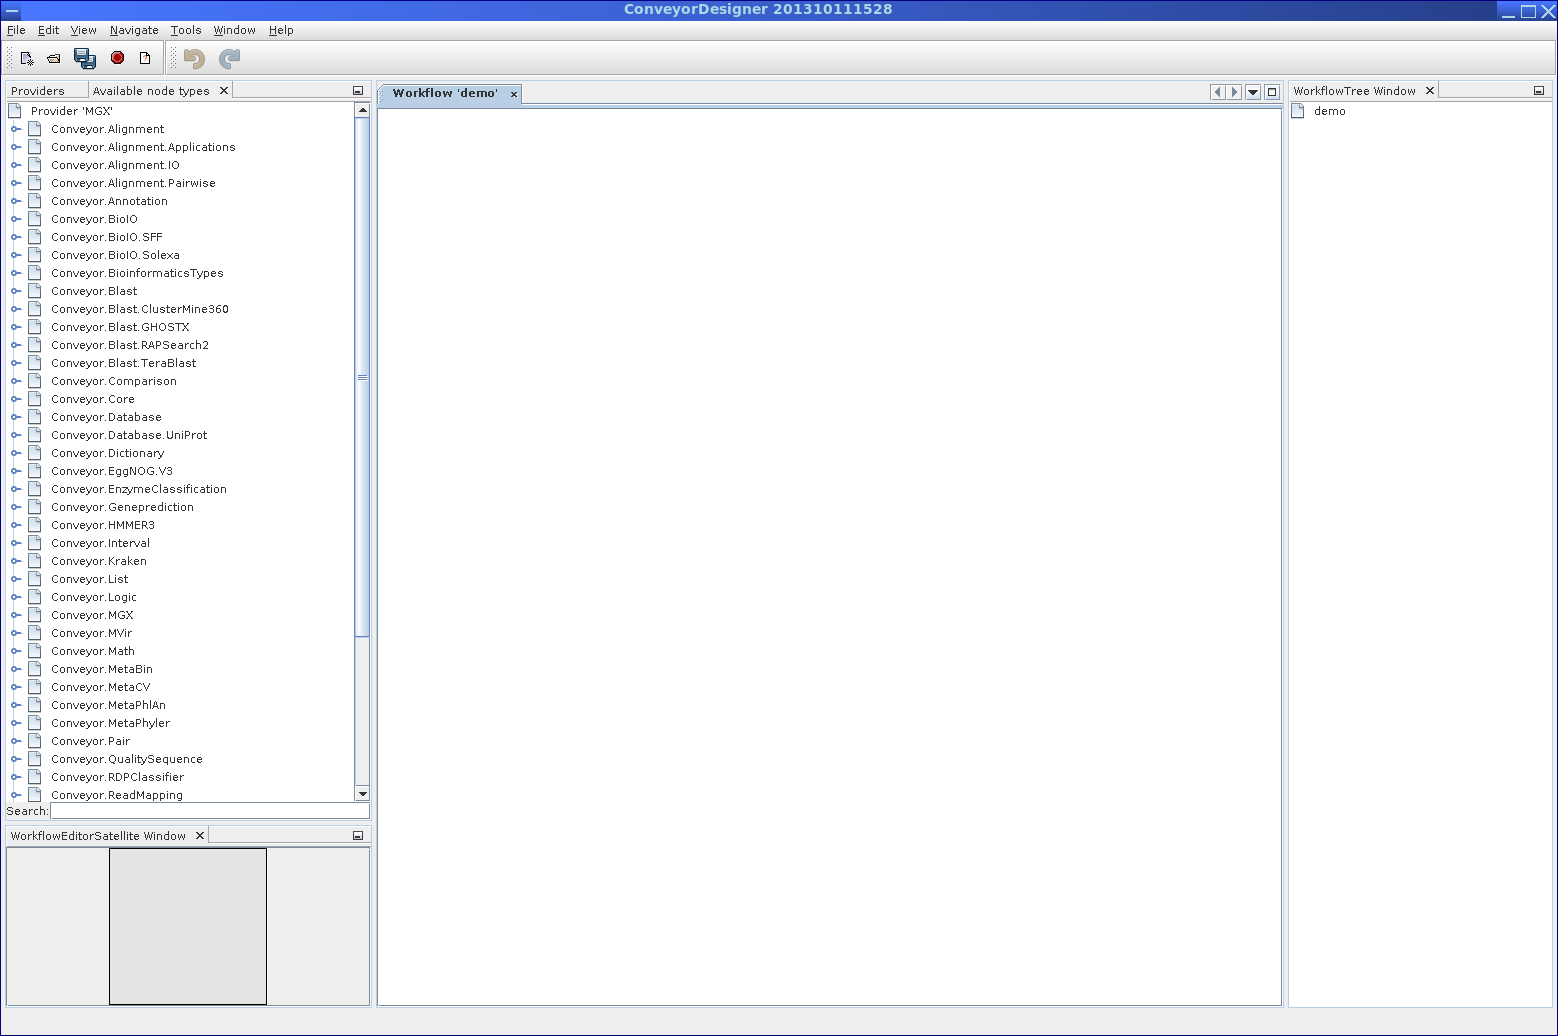
\includegraphics[width=\textwidth]{img/conveyor/designer}
\caption[Conveyor Designer]{The Conveyor Designer application allows easy and user-friendly
development of custom analysis algorithms in a graphical way.}
\label{designer}
\end{figure}

As Conveyor is actively developed and new tools are continously integrated, giving a thorough
introduction to Conveyor is beyond the scope of this document. The most up-to-date documentation describing
Conveyor itself and the Conveyor Designer in particular can be found at the Conveyor web
site \url{http://www.uni-giessen.de/fbz/fb08/bioinformatik/software/Conveyor}. 

\section{Getting started}

In order to implement a custom workflow, the Conveyor Designer needs to be configured
with a definition of available Conveyor plugins and node types. This is easily 
achieved by importing a plugin dump file, which contains a list of data types and
nodes provided by a Conveyor installation.

To use the Designer to implement a workflow for the MGX framework, a corresponding
plugin dump file can be obtained from within MGX by right-clicking on the 
project name (\ref{getdump}).

\begin{figure}[H]
\centering
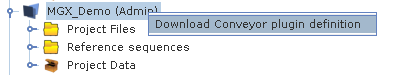
\includegraphics[width=.5\textwidth]{img/conveyor/getdump}
\caption[Plugin dump.]{A plugin dump file for use with the Conveyor Designer can be obtained from within MGX
by right-clicking on the project name.}
\label{getdump}
\end{figure}

Afterwards, start the Designer application and define a new provider (Right-click on ``Available providers''). 
Make sure to specify ``Plugin dump file'' (\ref{loaddump}) as the type of plugin set and select the file
generated by MGX. Once the plugin
dump file has been imported, you are ready to implement new workflows. Initially starting with an empty sheet,
nodes can be dragged from the list of all available nodes on the left and placed onto the sheet. Node connections
are created by clicking on a node, keeping the mouse button pressed and releasing it over the connections target
node, thus creating the link; in ambiguous cases, e.g. for nodes with several unconnected
inputs/outputs, a dialog will allow to select the desired connection.
Nodes may also require node-specific configuration, which can be edited from a nodes context menu.
A red border around a node indicates missing configuration items or connections.

\begin{figure}[H]
\centering
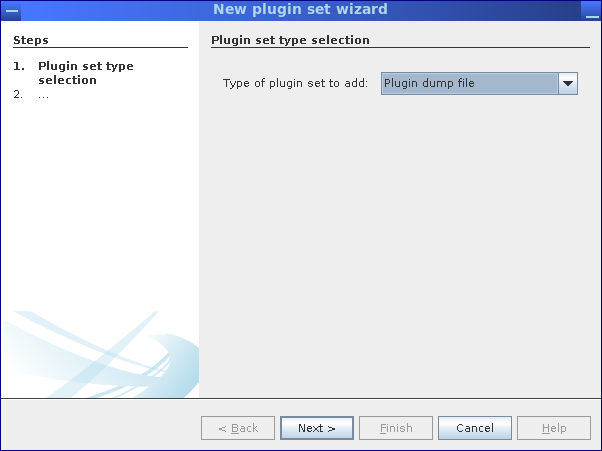
\includegraphics[width=.7\textwidth]{img/conveyor/loaddump}
\caption[Adding a new provider.]{Importing a plugin dump file into the Conveyor Designer.}
\label{loaddump}
\end{figure}

\section{Workflow requirements}

In order to design custom Conveyor workflows for later usage within the MGX platform, there
are several constraints to be met which will be described in more detail.\\

First of all, a dedicated \node{GetMGXJob} node (Figure \ref{getmgxjob}) has to be present within the workflow; in addition,
this node has to be named "\textbf{mgx}". During execution of a pipeline within MGX, this node is
configured via an external configuration file, providing required information about a jobs
context, like e.g. access to a project database and associated storage.\\

\begin{figure}[H]
\centering
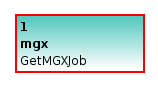
\includegraphics[width=.3\textwidth]{img/conveyor/getjob}
\caption[\node{GetMGXJob}]{The \node{GetMGXJob} node provides necessary context for executing a
workflow within MGX, such as database access. By convention, this node has to be named \textbf{mgx}.}
\label{getmgxjob}
\end{figure}

Access to metagenome DNA sequences is provided via the \node{ReadCSF} node, which will provide
all metagenome sequences for a sequencing run object within MGX, except those for which the 
``discard'' flag has already been set. As pipelines are always executed
for one single analysis job, this node needs to be connected to the \node{GetMGXJob} node (\ref{readcsf}).
Figure \ref{simple} shows a minimal example of a Conveyor-based pipeline for use within the MGX framework.
Once executed, the pipeline would set the \textit{discard} flag for all sequences.

\begin{figure}[H]
\centering
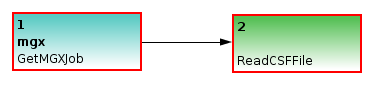
\includegraphics[width=.6\textwidth]{img/conveyor/getjobreadcsf}
\caption[\node{ReadCSF}]{The \node{ReadCSF} node is used to obtained metagenome sequence data 
from within MGX; it has one input and needs to be connected to the \node{GetMGXJob} node.}
\label{readcsf}
\end{figure}

\begin{figure}[H]
\centering
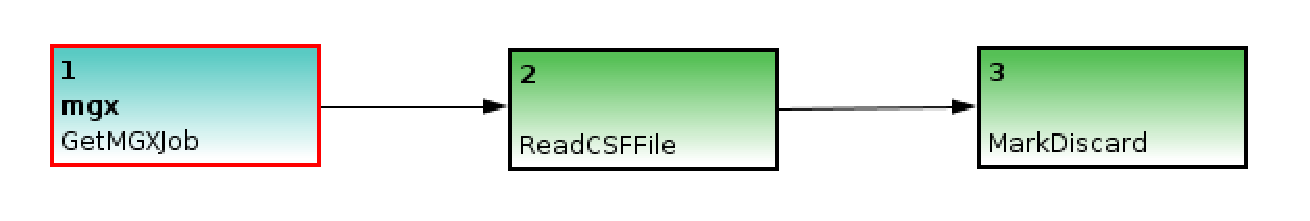
\includegraphics[width=.8\textwidth]{img/conveyor/simple}
\caption[Minimal example]{A minimal working example of a pipeline developed for MGX, which would set the \textit{discard} flag for all sequences.}
\label{simple}
\end{figure}


\section{Annotating metagenome sequences}

\begin{figure}[H]
\centering
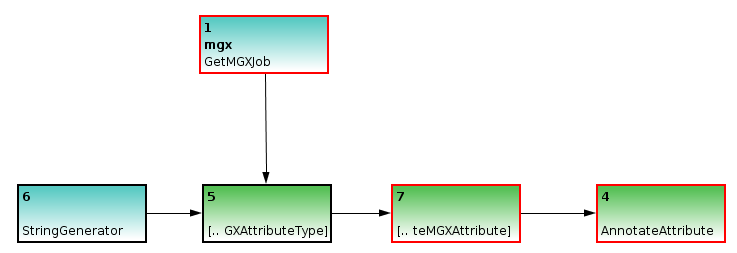
\includegraphics[width=.85\textwidth]{img/conveyor/annotate_templ}
\caption[Metagenome annotation]{Basic template to illustrate sequence annotation. A \node{StringGenerator} is
used to generate a label for the attribute type (\node{CreateMGXAttributeType}), which also requires job context
information. The attribute type is required to create attributes, thus the node is connected to the \node{CreateMGXAttribute} node. Finally, the annotation can be saved to the project database (\node{AnnotateAttribute} node).}
\label{annot}
\end{figure}

Annotation of metagenome sequences requires an ``attribute type'' and an ``attribute''. As an example, we will
illustrate the implementation of a pipeline for the analysis of GC content within metagenome sequences.
We use a \node{StringGenerator} node configured to generate the string ``GC'' to create a label for the
attribute type. As GC content is indicated by a number, we appropriately configure the \node{CreateMGXAttributeType}
node to emit a \textbf{basic} (i.e. not hierarchical) as well as numerical ``attribute type'' (\ref{createattrtype}).

\begin{figure}[H]
\centering
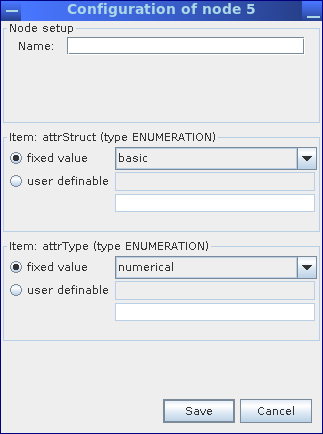
\includegraphics[width=.5\textwidth]{img/conveyor/createattrtype}
\caption[Defining an attribute type.]{Within the configuration dialog for the \node{CreateMGXAttributeType} node, structure and type of the generated attribute values are defined.}
\label{createattrtype}
\end{figure}

\begin{figure}[H]
\centering
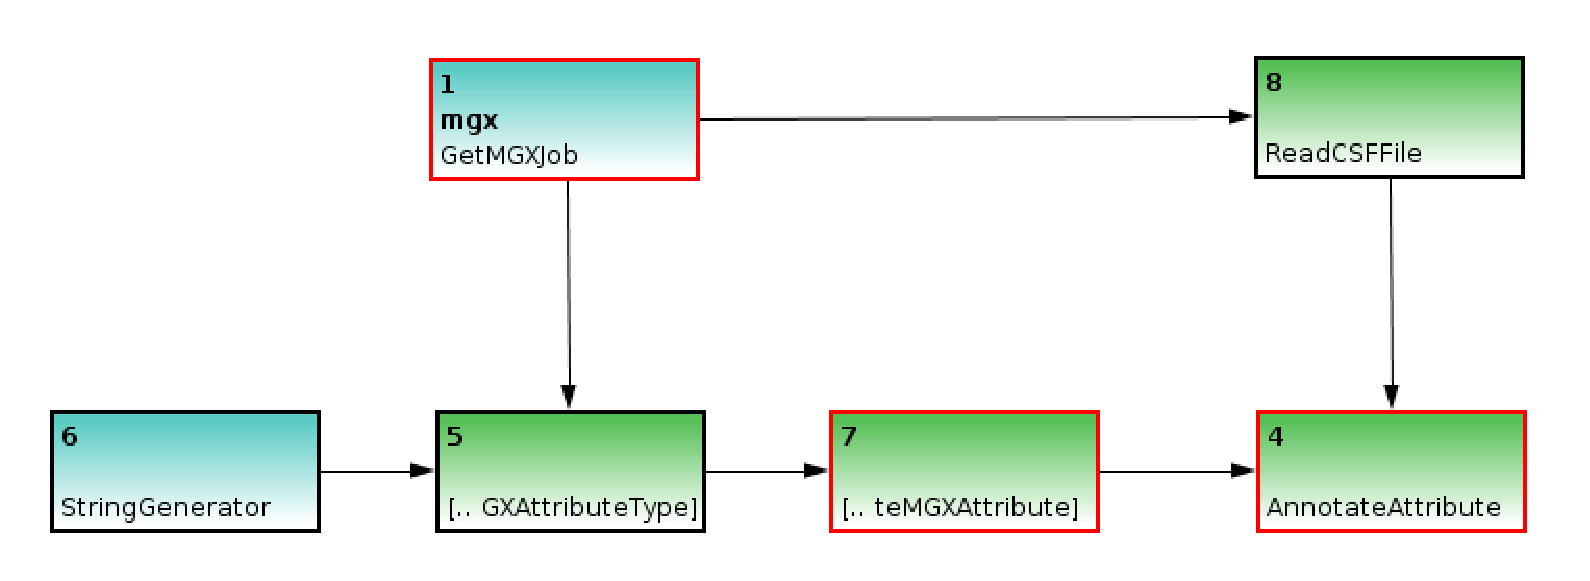
\includegraphics[width=.8\textwidth]{img/conveyor/annotate_templ2}
\caption[Metagenome annotation]{Incomplete example; extending upon \ref{annot}, the \node{ReadCSF} node will
provide the necessary metagenome sequences to be annotated. Still, there is no actual analysis specified.}
\label{annot2}
\end{figure}

In a second step, we use the \node{ReadCSF} node to obtain access to the individual metagenome sequences; as 
MGX annotates sequences individually, a connection between \node{ReadCSF} and \node{AnnotateAttribute} is
required (\ref{annot2}). Subsequently, we implement the actual analysis, which is provided by the \node{GCContent}
node. It will process all sequences and emit the corresponding GC content for each of them. To convert these values to
appropriate ``attributes'', an ``attribute type'' is required for each value; therefore, a \node{Repeat}
node is inserted between nodes 5 and 7 (\ref{annot3}).

\begin{figure}[H]
\centering
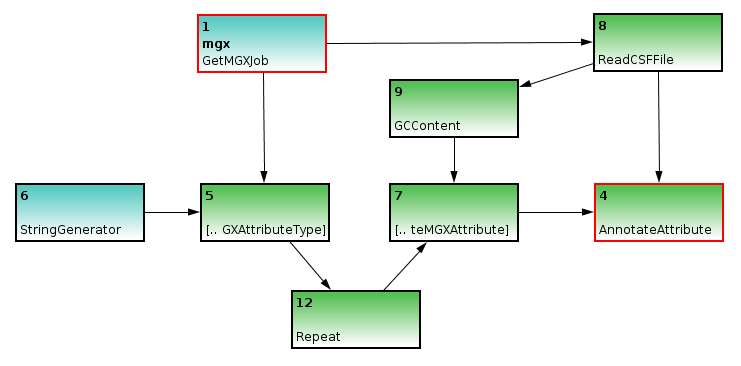
\includegraphics[width=.8\textwidth]{img/conveyor/annotate_templ3}
\caption[Metagenome annotation]{Step 2: The \node{GCContent} node represents the actual analysis step; it is used
to determine the GC content of a DNA sequence, which will then be converted into an ``attribute''. Since an 
``attribute type'' is required for each ``attribute'', a \node{Repeat} node is inserted between nodes 5 and 7.}
\label{annot3}
\end{figure}

Finally, as an annotation always refers to only a part of a sequence, we will need to generate the corresponding
start and end coordinates; since GC content refers to the full sequence, we can use an \node{ULongGenerator} node
configured to emit 0 (MGX uses 0-based coordinates) to generate the start coordinate; this node needs to be connected to
a \node{Repeat} node to generate a series of 0s.\\
The end coordinate can be created based on the sequences' length, with 1 subtracted, obtained through the
\node{GetLength} and \node{MinusOne} nodes (\ref{annot4}).\\
The \node{GetMGXJob} node will retain its red border due to missing configuration; this, however, can be
ignored, as appropriate configuration will be provided by the MGX framework automatically.

\begin{figure}[H]
\centering
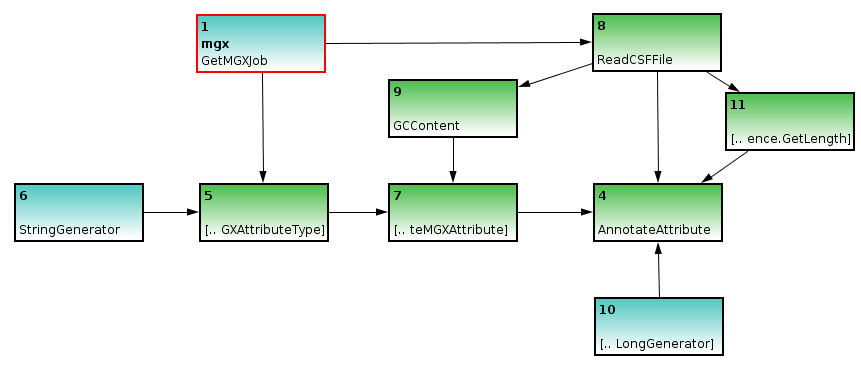
\includegraphics[width=.9\textwidth]{img/conveyor/annotate_templ4}
\caption[Metagenome annotation]{Completing the workflow: the \node{ULongGenerator} and \node{GetLength} nodes
are added to specify coordinates for the subregion of the DNA sequence described by the ``attribute''; the
start coordinate is simply repeated, while 1 is subtracted from the sequences length due to 0-based coordinates.}
\label{annot4}
\end{figure}

\subsection{Creating hierarchical attributes}

Annotation of hierarchical attributes requires a little more effort. The \node{CreateHierarchicalMGXAttribute} node
is used to obtain the inner structure of the hierarchy in a bottom-up approach; It contains several loops which
will be explained in more detail.

\begin{figure}[H]
\centering
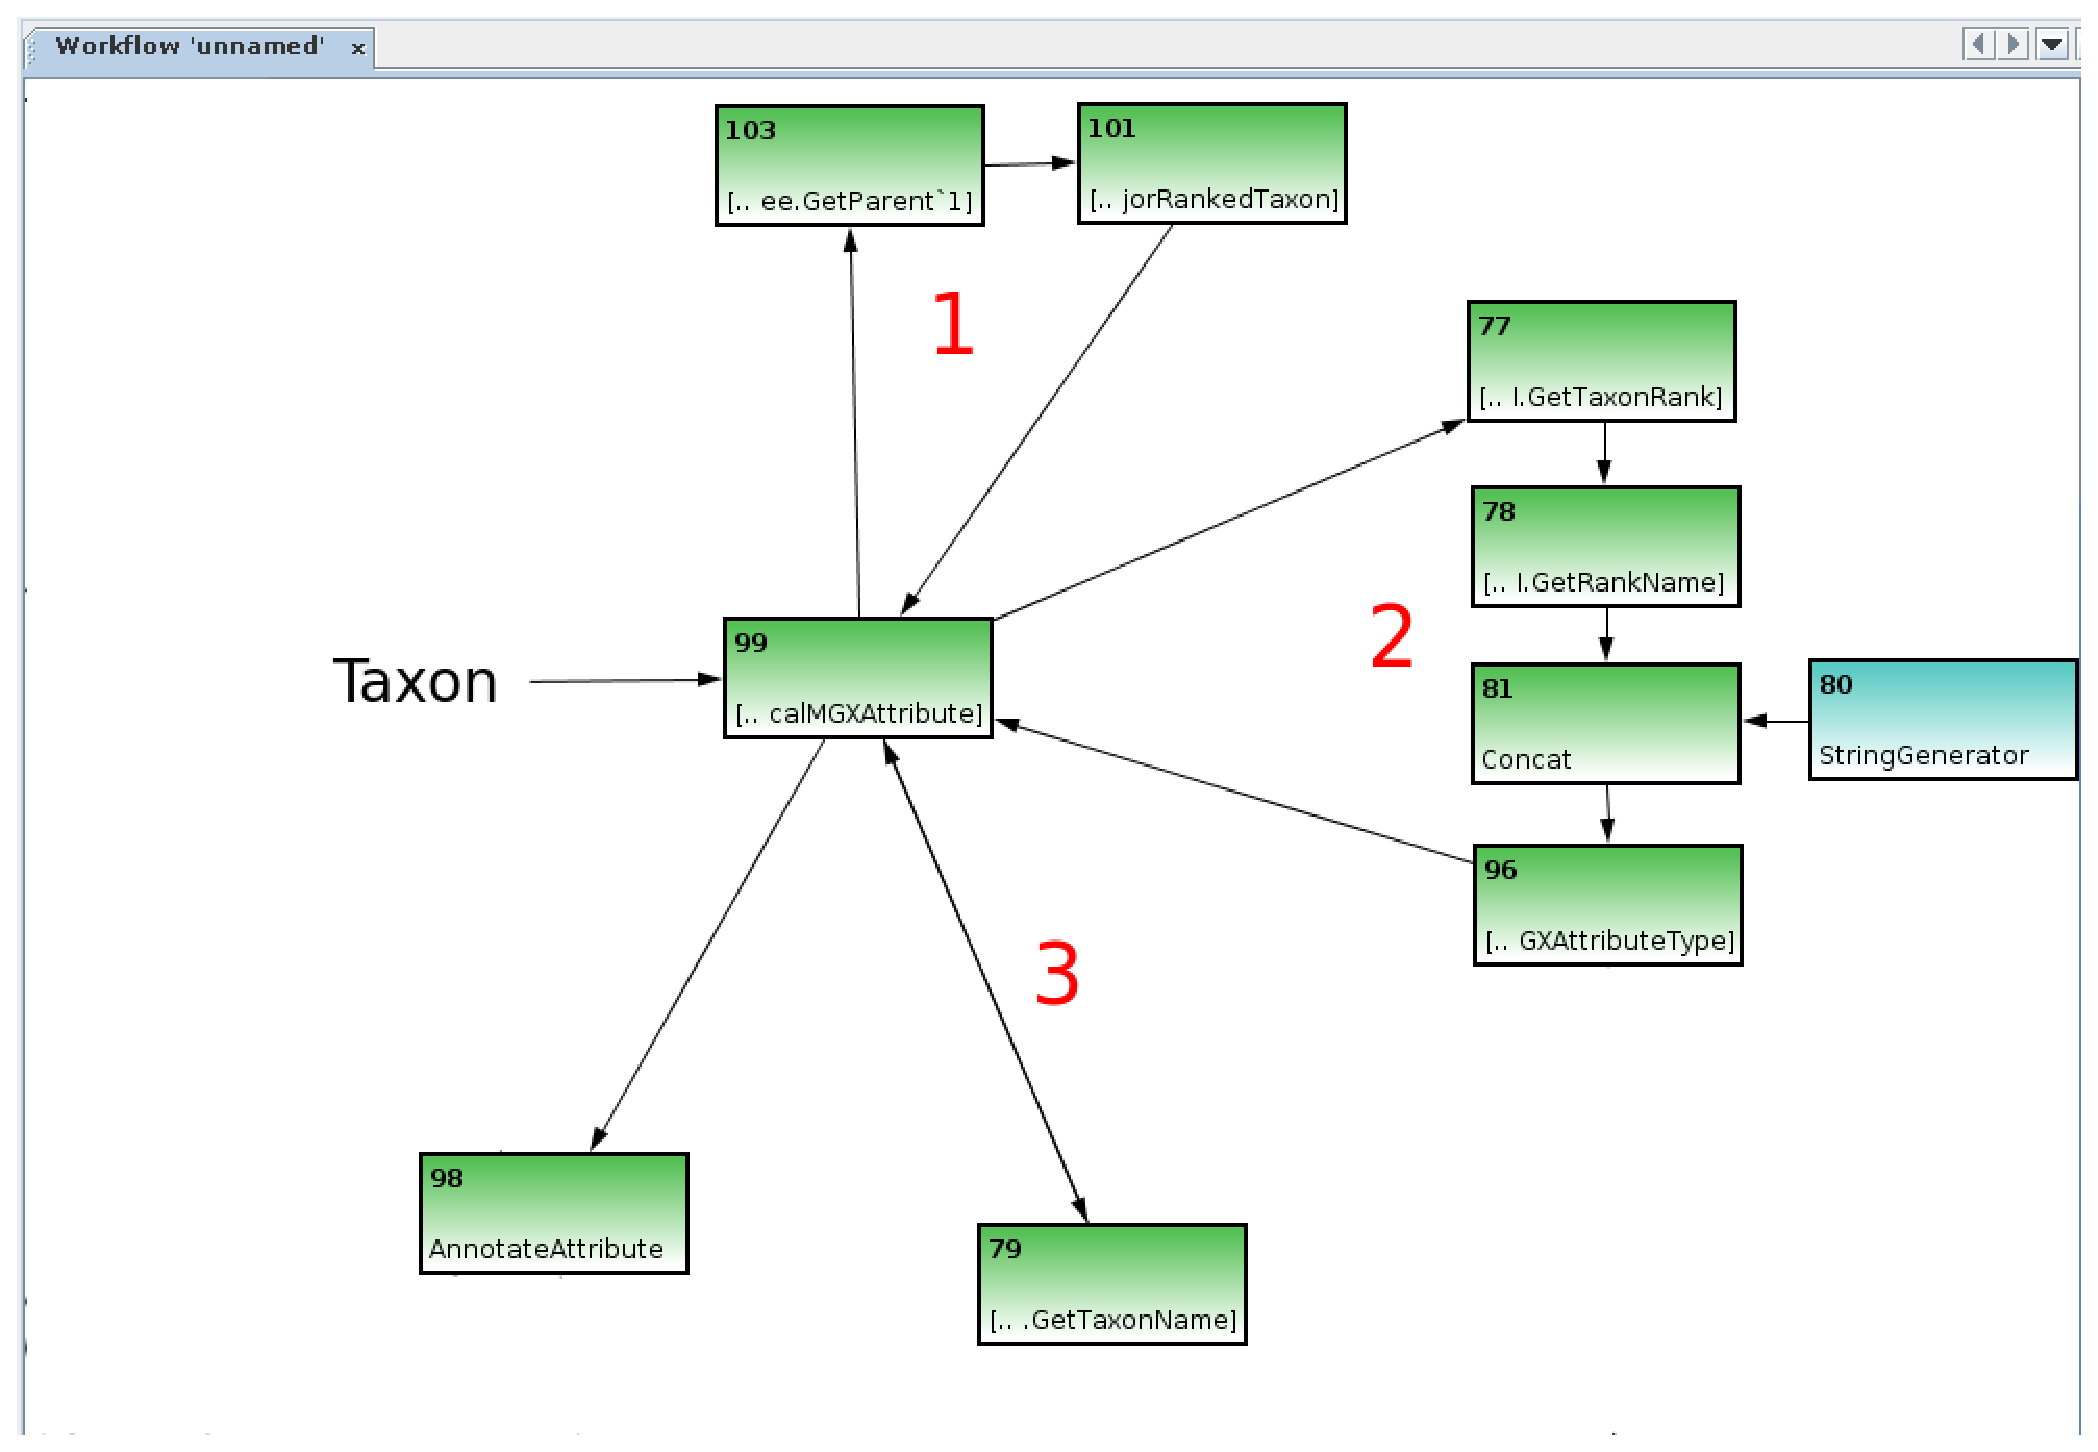
\includegraphics[width=\textwidth]{img/conveyor/TreeAnnot}
\caption[Hierarchical attributes]{The \node{CreateHierarchicalMGXAttribute} node requires three loops (note double-ended arrow on third loop)
to create the internal structure of the hierarchy. Several connections were removed from the figure
for illustrative purposes.}
\label{annot5}
\end{figure}

A single object, e.g. a NCBI taxon generated by the Kraken\cite{KRAKEN} classifier, is provided as an input
into the node (\ref{annot5}). 
The first loop is required to obtain the objects parent object, thus defining the hierarchy. In this example
it is implemented using the \texttt{GetParent} and \texttt{GetMajorRankedTaxon} nodes, thus making sure only
the major taxonomic ranks (superkingdom, phylum, class, \dots) are included.\\
The second loop is used to obtain the corresponding attribute type for an object: it operates on the initial taxon as well as its parents
obtained by the first loop. \texttt{GetTaxonRank} and \texttt{GetRankName} nodes provide the corresponding
ranks' name, e.g. ``class''; The \texttt{StringGenerator} and \texttt{Concat} nodes are then used to create the
attribute type: ``NCBI\_class''. This value is used to create the corresponding attribute type employing the
\node{CreateMGXAttributeType} node, which is returned into the \node{CreateHierarchicalMGXAttribute} node.\\
The third and final loop is used to map a data object to its name, which is used to create the attributes value;
it is built up using the \texttt{GetTaxonName} node, which delivers its output back into the node.\\

Thus, the three loops might be termed as \textbf{Get parent}, \textbf{Get AttributeType for object} and
\textbf{Generate value}. 

The \node{CreateHierarchicalMGXAttribute} node emits a hierarchical MGXAttribute for the initial data object,
with the corresponding AttributeType provided by loop 2 and the MGXAttribute's value obtained using loop 3.
Internally, loop 1 is used repetitively until the root node is reached, with all intermediary results
passing through loops 2 and 3, thus generating a single path of hierarchical attributes within the taxonomic
tree. The output of the \node{CreateHierarchicalMGXAttribute} is connected to the \node{AnnotateAttribute}
node as in the previous example.

For brevity's sake, several connections are hidden within the image, which have already been explained in the
previous section; the \node{CreateMGXAttributeType} node needs an incoming connection providing a MGXJob,
and the \node{AnnotateAttribute} node requires additional connections providing the sequence to be annotated
and start/stop coordinates for the subregion which is described by the annotation.



